\section{Design}

\textit{[I designkapitlet presenterar ni er implementation: skisser, lösningsförslag, hur lösningen utvecklats genom iterationer och motiverar era designbeslut med stöd från teori och resultat.]}

\textit{[Strukturera kapitlet så att det är tydligt hur designen utvecklats. Fokusera på de viktiga designbesluten och motivera dem. För mindre viktiga ändringar, hänvisa till bilagor.]}


\subsection{Designkoncept}

\textit{[Beskriv det övergripande designkonceptet]}

Det övergripande designkonceptet baseras på [beskriv huvudidé]. Gränssnittet riktar sig till [målgrupp] och ska främst stödja [huvudsakliga uppgifter].

Designen följer principerna om [t.ex. visibility, feedback, constraints från kurslitteraturen] för att säkerställa god användbarhet.


\subsection{Iteration 1: Tidiga skisser}

I den första iterationen skapades flera olika designalternativ. Figur \ref{fig:tidiga_skisser} och \ref{fig:tidiga_2}visar exempel på tidiga pappersprototyper.

\begin{figure}[H]
    \centering
    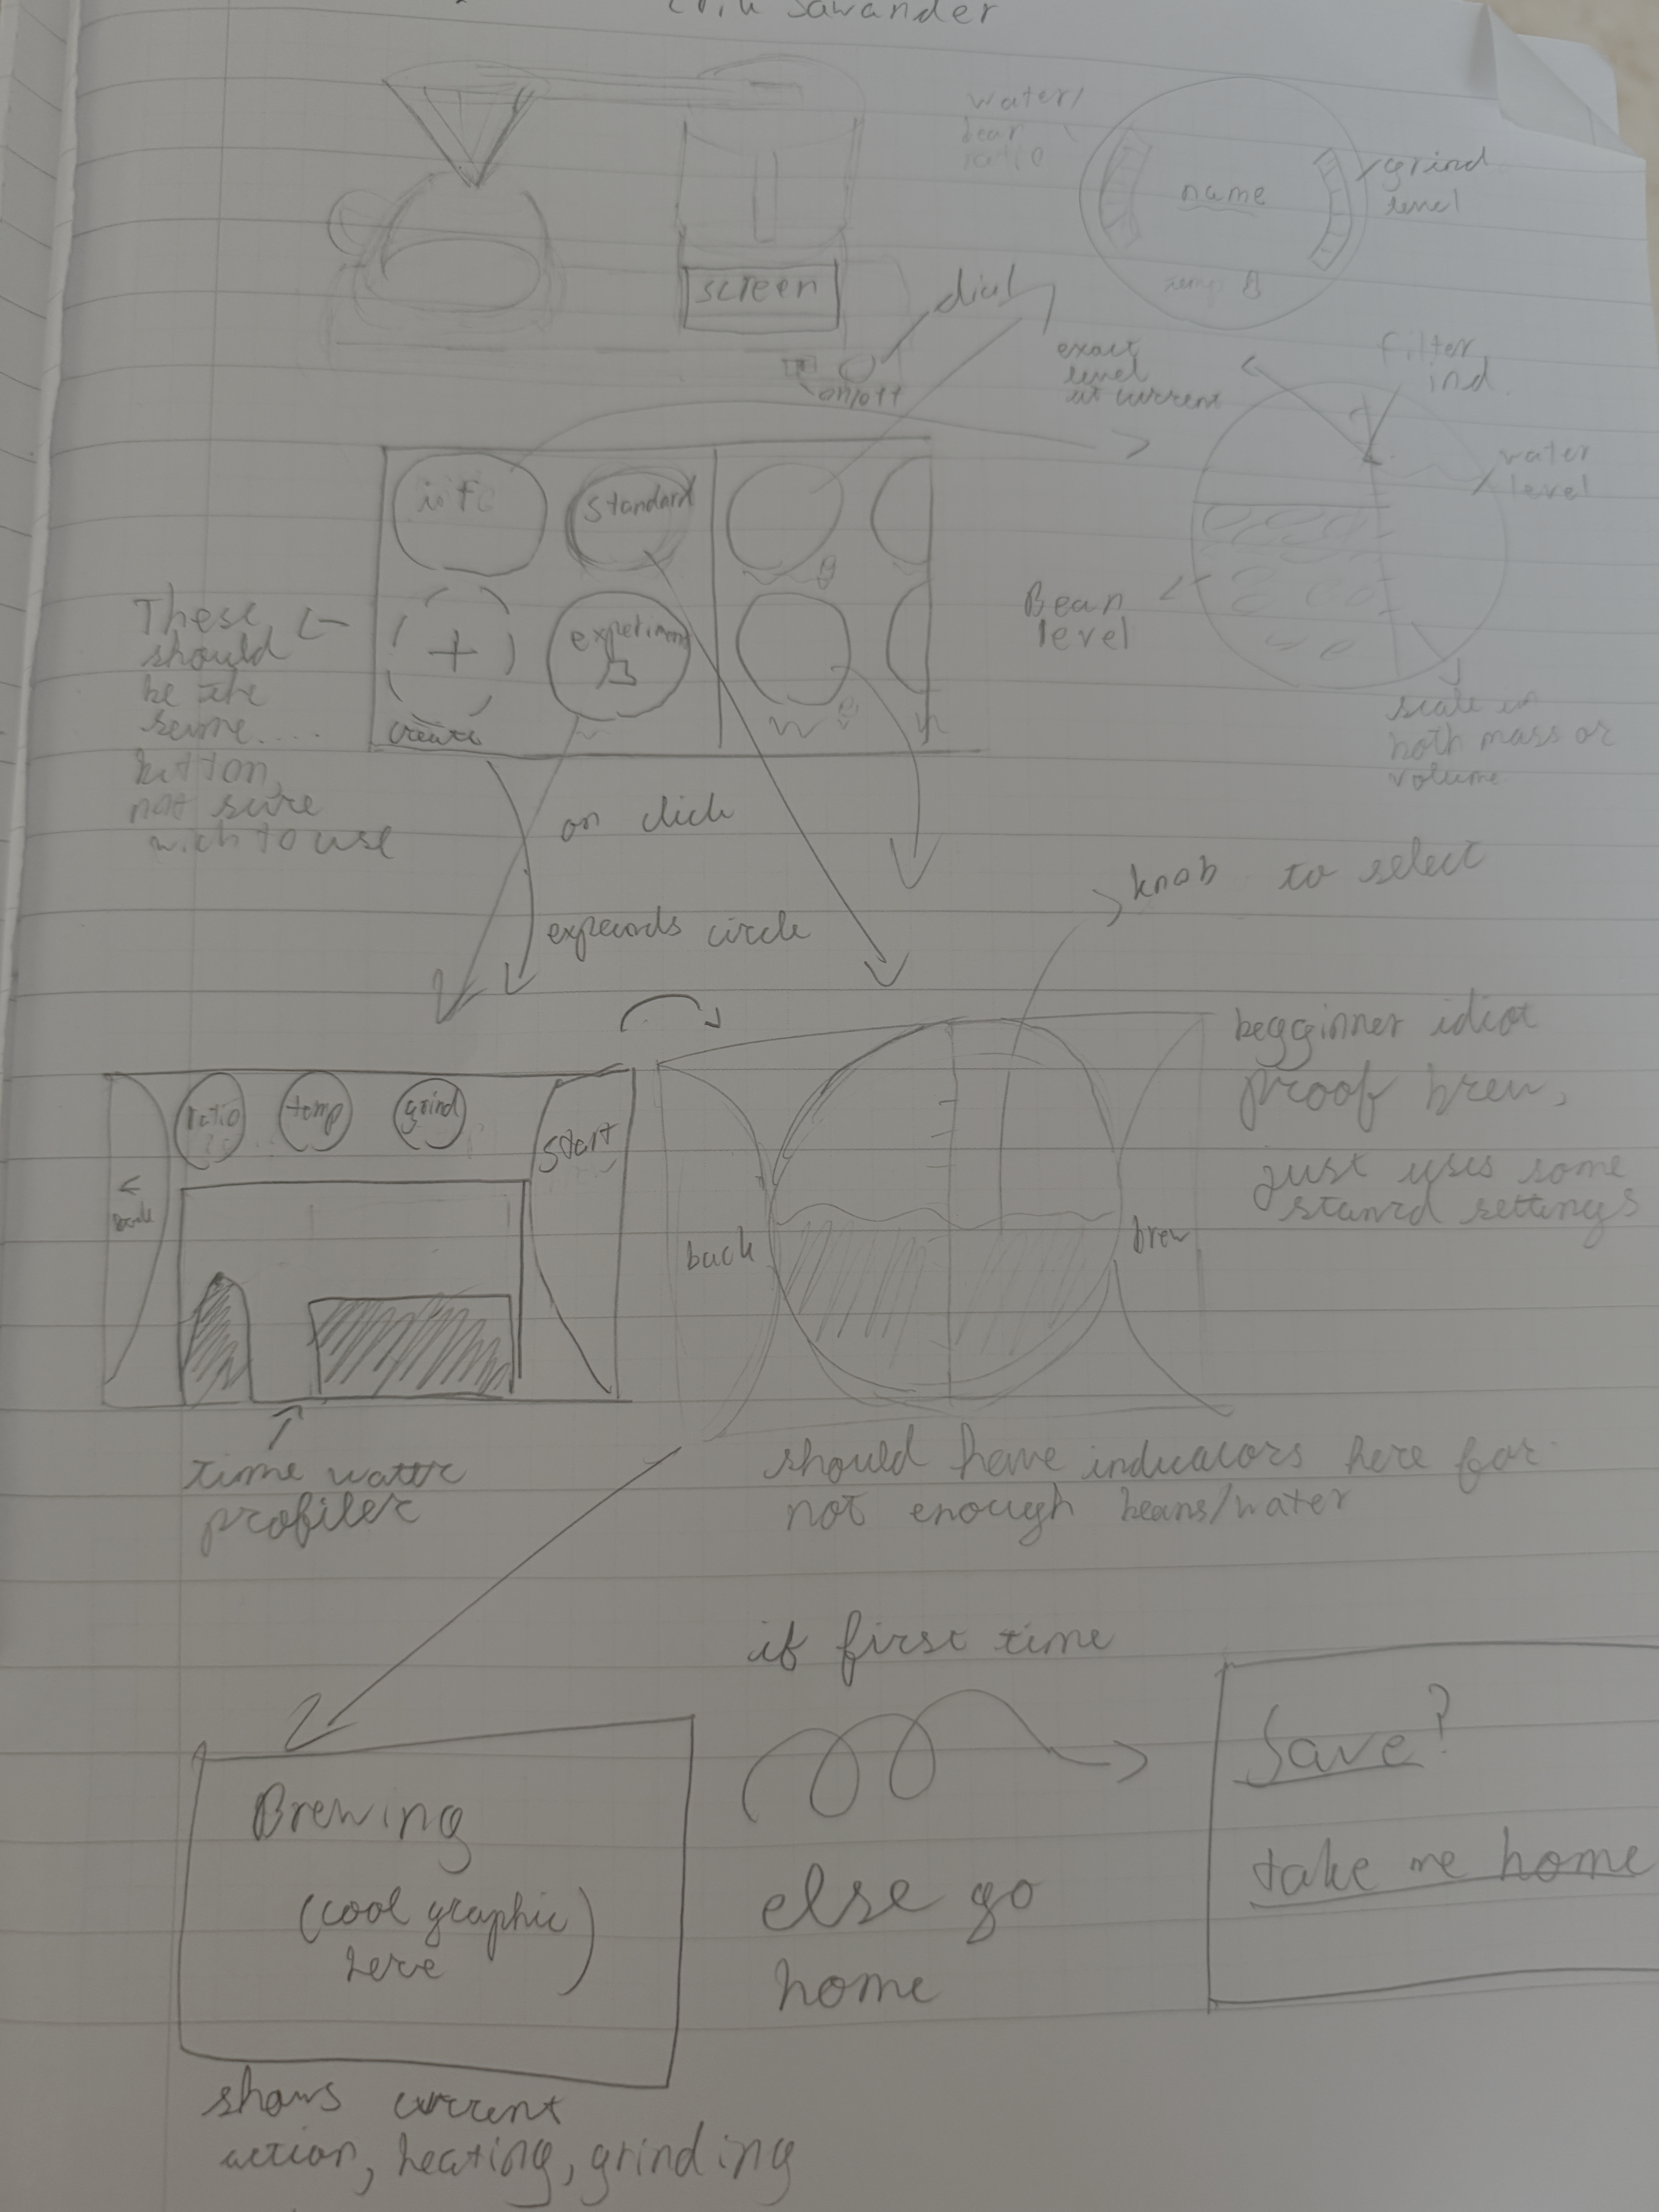
\includegraphics[width=0.8\textwidth]{bilder/paper.png}
    \caption{Tidig pappersprototyper från design studio-sessionen}
    \label{fig:tidiga_skisser}
\end{figure}

\begin{figure}[H]
    \centering
    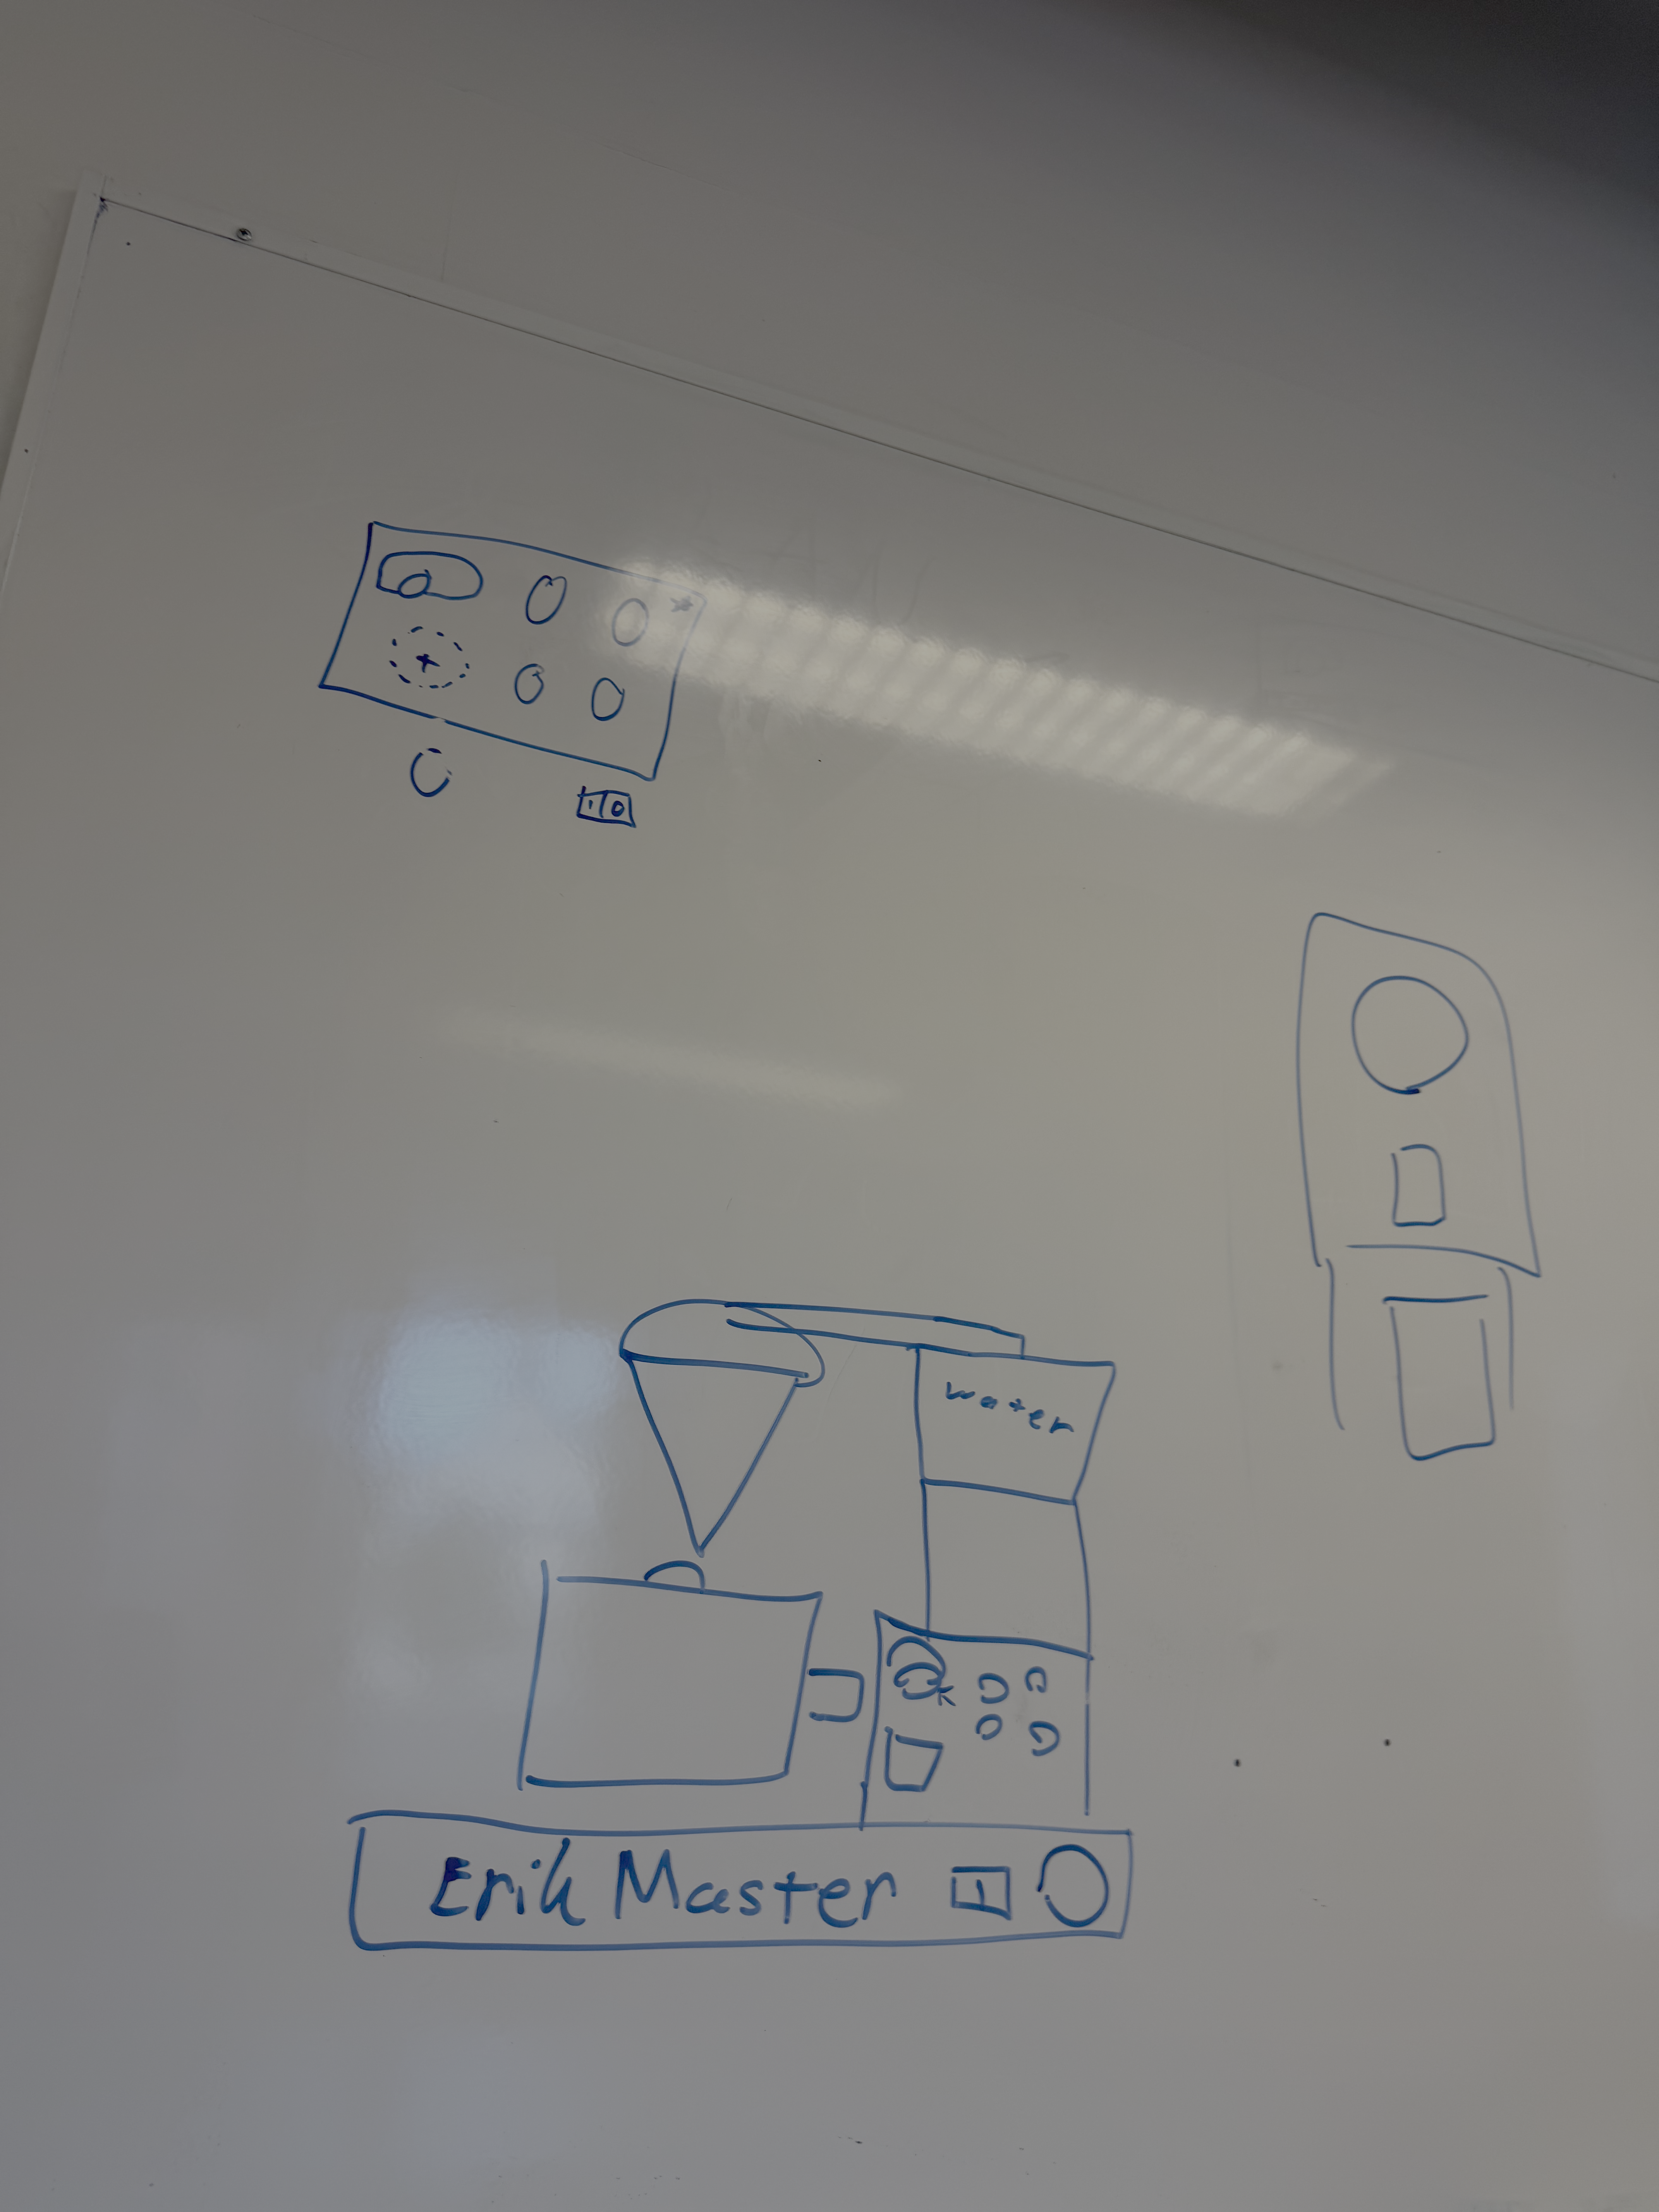
\includegraphics[width=0.8\textwidth]{bilder/whiteboard.png}
    \caption{Tidig prototyp från design studio-sessionen}
    \label{fig:tidiga_2}
\end{figure}

\textbf{Designalternativ A} fokuserade på... Detta alternativ valdes bort eftersom...

\textbf{Designalternativ B} erbjöd... Detta utvecklades vidare eftersom...


\subsection{Iteration 2: Första digitala prototyp}

\textit{[Beskriv utvecklingen till digital prototyp]}

Baserat på feedback från lo-fi-testerna utvecklades den första digitala prototypen. Huvudsakliga vyer inkluderar:

\subsubsection{Startsida}

\textit{[Beskriv varje viktig vy]}

Startsidan designades för att [syfte]. Layouten följer [designprincip] genom att...

\begin{figure}[h]
    \centering
    % \includegraphics[width=0.6\textwidth]{bilder/startsida_v1.png}
    \caption{Första versionen av startsidan}
    \label{fig:startsida_v1}
\end{figure}

Huvudelementen är:
\begin{itemize}
    \item \textbf{Navigation}: Placerad i [position] för att...
    \item \textbf{Sökfunktion}: Synligt placerad eftersom användarnas huvuduppgift är...
    \item \textbf{Content area}: ...
\end{itemize}


\subsubsection{[Annan viktig vy]}

\textit{[Fortsätt beskriva viktiga vyer]}


\subsection{Iteration 3: Förfinad design}

\textit{[Beskriv hur designen förbättrades baserat på utvärdering]}

Efter användbarhetstester i iteration 2 identifierades flera problem (se avsnitt \ref{sec:resultat_test}). Följande ändringar gjordes:

\textbf{Problem 1:} Användare hade svårt att hitta [funktion]

\textbf{Lösning:} [Funktion] flyttades till [position] och fick en mer framträdande visuell design (se figur \ref{fig:forbattring1}).

\begin{figure}[h]
    \centering
    % \includegraphics[width=\textwidth]{bilder/before_after.png}
    \caption{Före (vänster) och efter (höger) designändring}
    \label{fig:forbattring1}
\end{figure}

\textbf{Motivering:} Ändringen baseras på designprincipen om visibility \cite{sharp2019} och testresultaten visade att [beskriv förbättring].


\subsection{Slutgiltig design}

\textit{[Presentera den slutgiltiga designen]}

Den slutgiltiga designen är resultat av [antal] iterationer och integrerar feedback från [antal] användare. Fullständiga vyer finns i Bilaga C.

Huvudsakliga designprinciper som tillämpats:
\begin{itemize}
    \item \textbf{Konsistens}: Alla vyer följer samma layoutmönster...
    \item \textbf{Feedback}: Användaren får tydlig återkoppling när...
    \item \textbf{Affordance}: Interaktiva element signalerar tydligt...
\end{itemize}


\subsection{Designbeslut och motiveringar}

\textit{[Sammanfatta viktiga designbeslut]}

\begin{table}[h]
\centering
\begin{tabular}{|p{4cm}|p{5cm}|p{4cm}|}
\hline
\textbf{Designbeslut} & \textbf{Motivering} & \textbf{Teoretisk grund} \\
\hline
Navigation i top bar & Användarna förväntar sig... & Mental modeller \cite{sharp2019} \\
\hline
Färgschema: ... & Tillgänglighet och kontrast & WCAG-riktlinjer \\
\hline
... & ... & ... \\
\hline
\end{tabular}
\caption{Sammanställning av huvudsakliga designbeslut}
\end{table}
